\chapter{Introduction}

\section{Motivation}

% Hand-drawn \acp{ECD} are widely used in engineering, especially for the early design phases \cite{early_design}.

\acp{ECD} are used in electrical engineering to represent the functionality of an electrical circuit visually.
In early design phases, especially hand-drawn sketches of \acp{ECD} are used to get an initial concept of the underlying problem.
Engineers have more time to concentrate on the problem than on the design in \ac{CAD} programs.
In general hand-drawn methods are considered to be 90\% more time-efficient than \ac{CAD} methods \cite{ecd_ctxindependentsvm}.
When studying electrical engineering or related fields, students often have to draw sketches of \acp{ECD} and calculate the physical properties of the \acp{ECC} in the circuit.
The complexity of the calculations grows with the circuit's size and also depends on the used \acp{ECC}.
For example, when sources with auxiliary properties are used, calculations become dependent on the frequency of the sources, which adds additional complexity.
In the real world, such calculations are normally done in a circuit simulation software such as LTspice.
Here, the circuit is designed with its \acp{ECC} and their physical properties.
Parameters of interest can then be obtained by simulating the circuit in that program.
While the simulation of a circuit is fast and the parameters of interest can be obtained fast, designing a circuit in such a program is generally slower than drawing it by hand.

To increase the efficiency of engineers and students in designing and verifying their calculations respectively, a method to convert an image of a hand-drawn \ac{ECD} could ease the use of \ac{CAD} software and circuit simulation software.

\section{Problem Statement}
\label{sec:problem_statement}

To understand how a conversion of a hand-drawn \ac{ECD} into a digital format can be achieved first, the various components of an \ac{ECD} have to be presented.
Typically, an \ac{ECD} consists of \acp{ECC}, where for each \ac{ECC}, a unique symbol is defined in the international standard \cite{iec60617}.
\acp{ECC} are connected with lines, which correspond to wires in the real world.
Wires and \acp{ECC} together form the topology of the underlying circuit.

Additionally, \acp{ECC} can be further be specified by an annotation next to their symbol, which consists of a digit followed by a unit.
This annotation determines the physical properties of the underlying \ac{ECC}.
Voltage sources and current sources are annotated with an arrow next to their symbol, which indicates the direction of the potential difference or, in the latter case, the direction of the current flow.

Furthermore, it is common that \acp{ECD} are drawn on gridded paper since it provides a simple way to align the different components. An example of an \ac{ECD} drawn on grid paper with its \acp{ECC} and annotations can be seen in figure \ref{fig:example_ecd}.

\begin{figure}
\begin{center}
    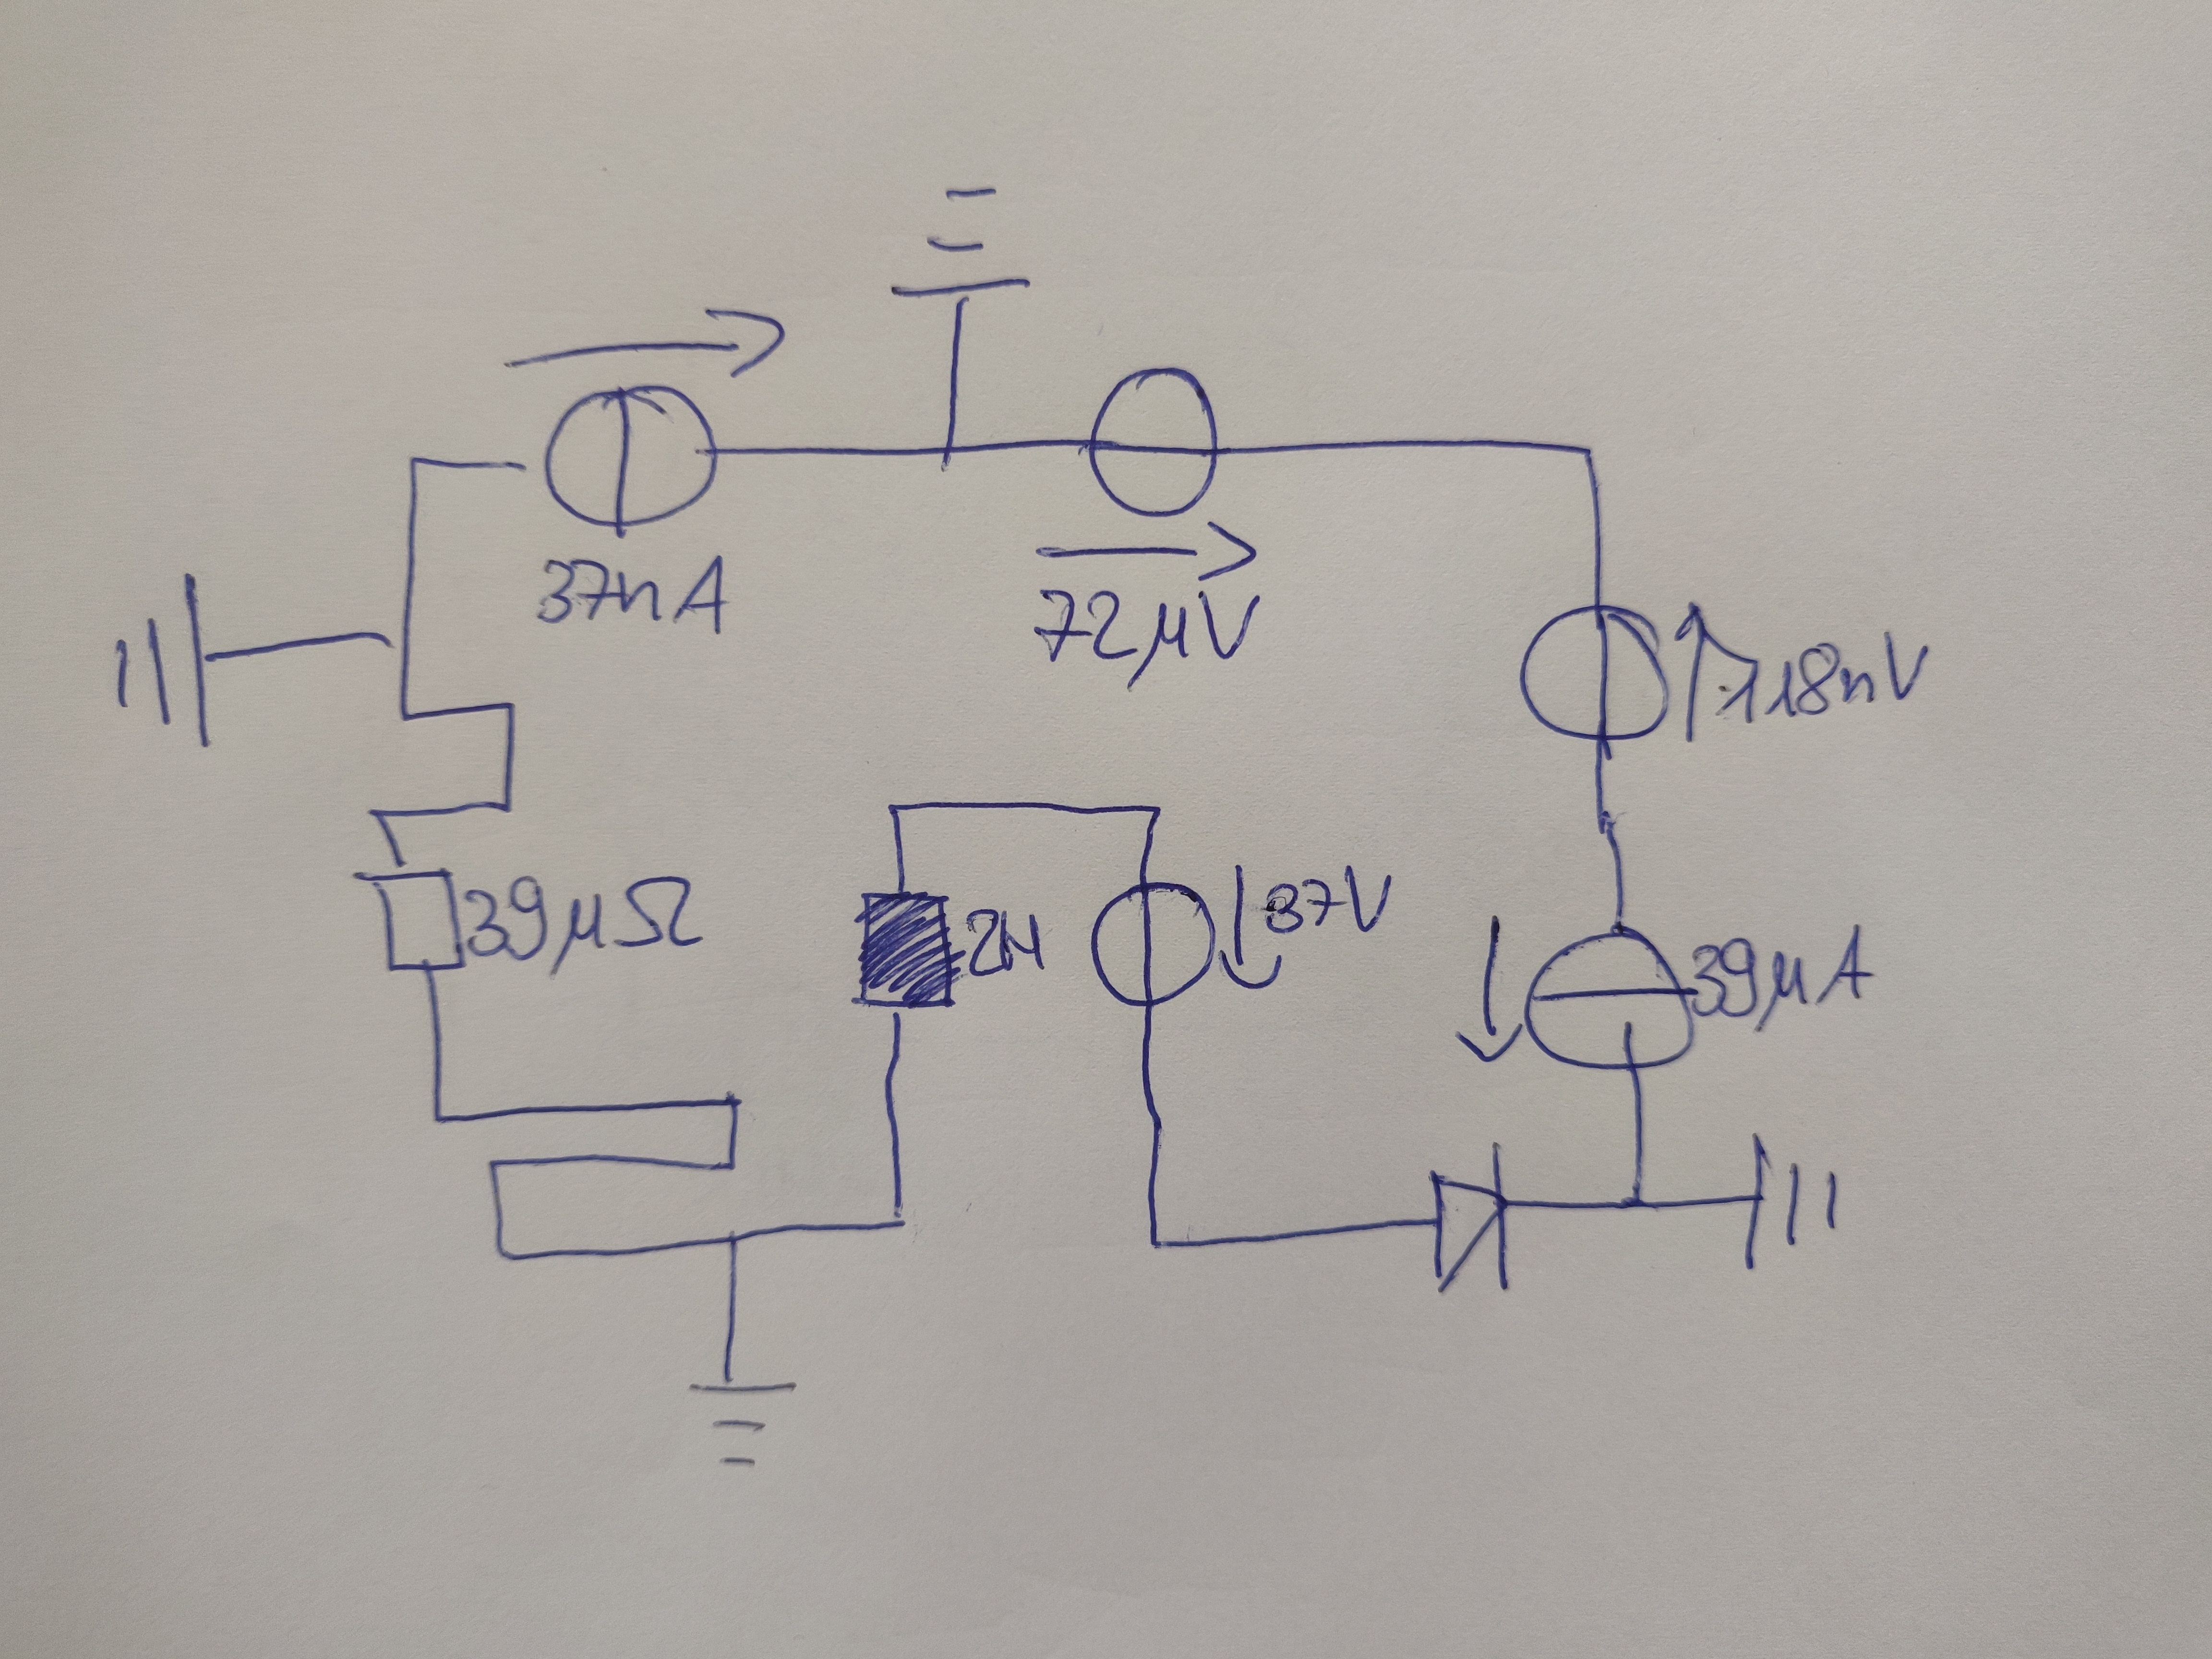
\includegraphics[width=11cm]{imgs/eccs/ecd.png}
    \caption{A drawing of an \ac{ECD} on a grid paper background with its \acp{ECC} and annotations.}
    \label{fig:example_ecd}
\end{center}
\end{figure}

\newpage
So a conversion pipeline has to be able to capture all of the above properties of an \ac{ECD}.
To achieve this the necessary subtasks have been identified as follows:
\begin{enumerate}
    \item Detect the class and position of an \ac{ECC} and its annotations
    \item Match annotations to their respective \ac{ECC}
    \item Interpret the text in the textual annotations
    \item Detect the topology of the \ac{ECD}, regardless of the used paper background
    \item Embed the information into the target format
\end{enumerate}

\section{Related Work}

To provide some context for the task at hand, in the following related approaches to the goal of this thesis are presented.
The gathered works can be structured into three categories:
\begin{enumerate}
    \item Classification of \acp{ECC} and related components (section \ref{sec:rel_classification}).
    \item Extraction of \acp{ECC} from an image of an \ac{ECD} with following classification (section \ref{sec:rel_extract_classification}).
    \item Extraction of all related information from \acp{ECD} or related structured diagrams and classification of the components (section \ref{sec:rel_extract_classification_topology}).
\end{enumerate}

\subsection{Classification}
\label{sec:rel_classification}

G"unay et al. \cite{ecd_basecnn} compared in their work the accuracy of various common \ac{CNN} architectures trained on a dataset of hand-drawn \acp{ECC}.
The dataset consisted of four classes (resistor, capacitor, inductor, voltage source) and had overall a size of 863 images.
With the best performing \ac{CNN} architecture, they were able to obtain an accuracy of 83\%.

Rabbani et al. \cite{ecd_anngeo} tested the classification performance of letters, numbers, and \acp{ECC} in their work.
For each class, a total of 20 samples was used.
The classification was done using a \ac{MLP}, where different geometric and moment features were fed into the network.
Overall they reported an f1-score of 83.5\%.

Roy et al. \cite{ecd_texturesmo} used in their dataset 20 different \acp{ECC} with around 150 samples per class.
As a classifier, \ac{SMO} was used, which was fed with different features based on texture and shape.
Further, they compared the performance of the \ac{SMO} classifier to the Random Forest classifier, an \ac{MLP}, a \ac{KNN} classifier, and the Naive Bayes classifier.
An accuracy of 91.88\% was reported for the \ac{SMO} classifier.


\subsection{Extraction and Classification}
\label{sec:rel_extract_classification}

Dewangan and Dhole \cite{ecd_knn_recog} proposed a pipeline that can extract \acp{ECC} from an \ac{ECD} and classify it.
The initial step was formed by a preprocessing pipeline, which binarized the image, denoised it, and then skeletonized it.
Afterwards, segmentation was used to segment wires and components individually.
The segmentation has not been described in full depth, thus no detailed insights can be given at this point.
Finally, based on the segmented \acp{ECC}, numerous features were obtained like area, major axis length, minor axis length, centroid, orientation, eccentricity, convex area, filled area, equiv diameter, and extent.
Those features were used to train a \ac{KNN} classifier, where an accuracy of 90\% was reported.

Moetesum et al. \cite{ecd_seghogsvm} proposed a similar pipeline.
A dataset of 100 images of \acp{ECD}, which contained a total of ten different classes, with 35 samples per class, was used.
With a total amount of 350 samples, 200 were used for training and 150 for testing.
Preprocessing was done by first converting the image to grayscale, denoising with a smoothing filter, followed by binarization of the image.
Afterwards, the \acp{ECC} were segmented using different strategies based on the shapes of the \acp{ECC}.
For example, diodes were segmented using the assumption that the shape is closed, and capacitors were segmented using its parallel line property.
Afterwards, \ac{HOG} features were obtained from the segmented components, which were then fed into a \ac{SVM}.
An accuracy of 87.71\% was reported on the whole dataset, where the evaluation was done using transient errors, i.e., an error produced in the segmentation will automatically produce an error in the classification since the component could not be segmented and hence also not classified.

\subsection{Extraction, Classification and Topology Creation}
\label{sec:rel_extract_classification_topology}

Edwards and Chandrun \cite{ecd_knnfull} proposed a pipeline to create an \ac{ECD} from a hand-drawn image into a digital form.
The dataset comprised 449 \acp{ECC} and 107 nodes, where a node is defined as a connection or set of connections.
In the preprocessing step, first a grayscale conversion was performed, followed by noise reduction and image binarization.
To mitigate common errors such as small gaps in lines, morphological closing was performed, and the number of pixels per region was normalized through a thinning algorithm.
In the next step, the \acp{ECC} and connections were segmented, based on the pixel density in a region.
Here the assumption was that plain lines (wires) will have a lower pixel density inside a small circular region than \acp{ECC} or connections and with an appropriate threshold, they could be segmented.
Classification of the segmented components was performed with a \ac{KNN} classifier, which classifies different geometric and moment features of the segmented regions.
To recreate the topology, the connections between the \acp{ECC} had to be identified.
This was done using the Breadth-First Search algorithm, which started at a certain component and tried to find a path to another one.
When a path was found, it indicated a connection between those two components.
Finally, a node recognition accuracy of 92\% and a classification accuracy of 86\% were reported.

Refaat et al. \cite{ecd_ctxindependentsvm} proposed a context-independent approach for structured diagram recognition utilizing \acp{SVM}.
Their dataset was comprised of graphics, which were basic line primitives such as rectangles, circles, triangles, ellipse, and text annotations, as well as lines connecting the graphics.
The preprocessing consisted of an adaptive thresholding approach to separate the foreground from the background.
Segmentation was performed based on size filters to segment the text annotations, which were relatively small compared to the graphics.
To segment the graphics and lines, a model was used, which imitates the human perception of shapes based on the smoothness and continuity property.
The used algorithm can be found in \cite{line_primitive}.
After segmentation, the shapes were classified using an \ac{SVM} classifier that was trained with 120 images of each shape.
For testing, 20 images per shape were used, and a classification accuracy of 90\% was reported.

Dhanushika and Ranathunga \cite{ecd_yolobool} proposed an approach that can provide a boolean expression from an image of a logical gate diagram.
Their dataset consisted of 300 diagrams, where 240 were used for training, and 60 were used for testing.
To detect the logical gate components, two different object detection networks were presented.
They trained a \ac{YOLO} network and a network from the open-source deep learning framework TensorFlow \cite{tensorflow} (the exact network was not mentioned).
Detection of connections between components was done using a rule-based approach.
First, the lines were extracted using the Hough Transform \cite{hough_transform} and vertical and horizontal lines were split up in different chunks.
Afterwards, intersections were calculated between the lines of the chunks, and different patterns were identified based on the proposed rules.
For example, a pattern for an edge was identified or for a ``T'' connection, which indicates that three components are connected at this particular connection.
By starting from a logical gates component and tracing along the identified pattern, it could be identified whether two (or more) components were connected.
From the gathered results, a boolean expression could then be generated.
Three different metrics were reported based on the different detection types.
For the \ac{YOLO} network, an accuracy of 40\%  was reported, while for the unknown TensorFlow object detection algorithm, an accuracy of 90\% was reported.
Further, for the line and connection detection, an accuracy of 83.11\% and 89.49\% were reported, respectively.

\section{Goals of this Thesis}

\subsection{Task Description}

In section \ref{sec:problem_statement}, the subtasks at hand were presented, which are required to achieve a conversion pipeline.
In this section, each subtask is presented with a technical solution, which will briefly be described in the following.
Identifying the class and position of the \acp{ECC} and annotations is essentially an object detection problem.
Therefore, the object detection network \ac{YOLO} will be used to identify those.
Detecting the topology will be done by combining various computer vision methods in a specifically tailored algorithm.
Here also, the emphasis should be put on the different paper backgrounds, which can be handled by a neural network dedicated to the segmentation task, more precisely the \ac{MUnet}.
Further, a simple algorithm will be introduced, which allows the matching of annotations to their respective \ac{ECC}.
The interpretation of the textual annotations is the only step that is not handled, but could be solved by an \ac{OCR} engine such as Tesseract \cite{tesseract}.
The last step will be the embedding of the information into an output format, which will be demonstrated based on the LTspice schematic file format.

\subsection{Contribution}

The contributions of this work can be summarized as follows:

\begin{itemize}
    \item Creation of a dataset of \acp{ECD}, with \acp{ECC} in German notation (section \ref{sec:data}).

    \item A pipeline that receives an image of an \ac{ECD}, either on white or grid paper, classifies the components and returns a schematic file for LTspice as output (section \ref{sec:pipeline}).

    \item A systematic ablation study-like parametrization of the two branches of the proposed pipeline:
    \begin{itemize}
        \item \ac{ECC} Detection: \ac{YOLOv4}-Tiny (section \ref{sec:training_yolo})
        \item \ac{ECD} Segmentation: \ac{MUnet} (section \ref{sec:training_munet})
    \end{itemize}

    \item The proposal of an evaluation algorithm measuring the similarity between two detected topologies (section \ref{sec:eval_algo}).

    \item An evaluation of the proposed pipeline with the proposed evaluation algorithm (section \ref{sec:evaluation_results}).
\end{itemize}
